% Created by tikzDevice version 0.12.3.2 on 2023-05-16 17:29:55
% !TEX encoding = UTF-8 Unicode
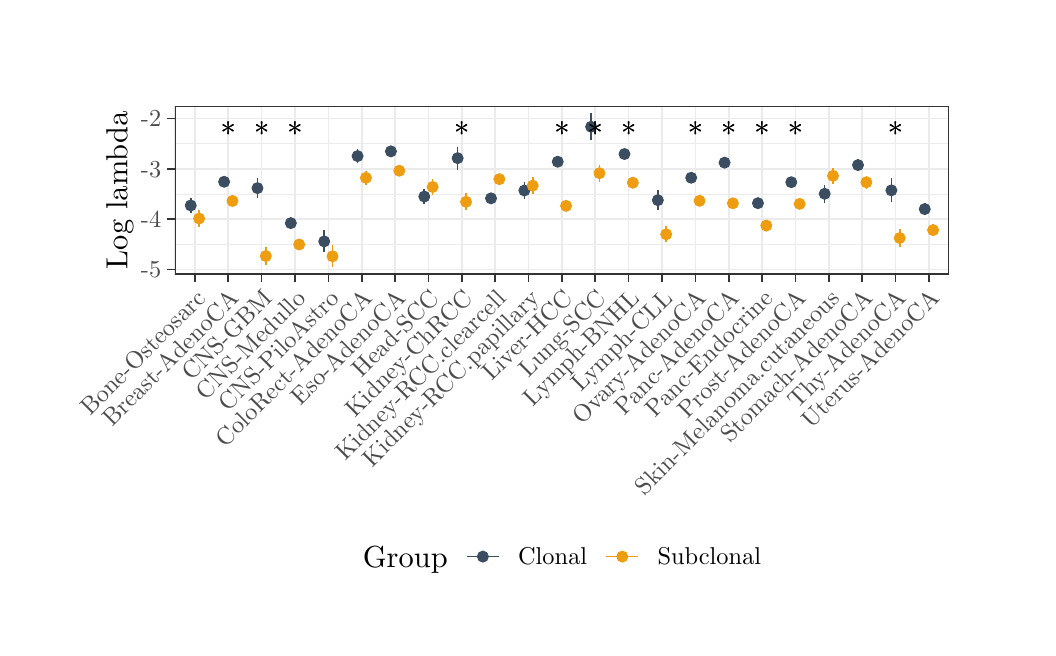
\begin{tikzpicture}[x=1pt,y=1pt]
\definecolor{fillColor}{RGB}{255,255,255}
\path[use as bounding box,fill=fillColor,fill opacity=0.00] (0,0) rectangle (361.35,216.81);
\begin{scope}
\path[clip] (  0.00,  0.00) rectangle (361.35,216.81);
\definecolor{drawColor}{RGB}{255,255,255}
\definecolor{fillColor}{RGB}{255,255,255}

\path[draw=drawColor,line width= 0.6pt,line join=round,line cap=round,fill=fillColor] (  0.00,  0.00) rectangle (361.35,216.81);
\end{scope}
\begin{scope}
\path[clip] ( 53.20,127.70) rectangle (332.90,188.36);
\definecolor{fillColor}{RGB}{255,255,255}

\path[fill=fillColor] ( 53.20,127.70) rectangle (332.90,188.36);
\definecolor{drawColor}{gray}{0.92}

\path[draw=drawColor,line width= 0.3pt,line join=round] ( 53.20,138.51) --
	(332.90,138.51);

\path[draw=drawColor,line width= 0.3pt,line join=round] ( 53.20,156.71) --
	(332.90,156.71);

\path[draw=drawColor,line width= 0.3pt,line join=round] ( 53.20,174.91) --
	(332.90,174.91);

\path[draw=drawColor,line width= 0.6pt,line join=round] ( 53.20,129.41) --
	(332.90,129.41);

\path[draw=drawColor,line width= 0.6pt,line join=round] ( 53.20,147.61) --
	(332.90,147.61);

\path[draw=drawColor,line width= 0.6pt,line join=round] ( 53.20,165.81) --
	(332.90,165.81);

\path[draw=drawColor,line width= 0.6pt,line join=round] ( 53.20,184.01) --
	(332.90,184.01);

\path[draw=drawColor,line width= 0.6pt,line join=round] ( 60.43,127.70) --
	( 60.43,188.36);

\path[draw=drawColor,line width= 0.6pt,line join=round] ( 72.49,127.70) --
	( 72.49,188.36);

\path[draw=drawColor,line width= 0.6pt,line join=round] ( 84.54,127.70) --
	( 84.54,188.36);

\path[draw=drawColor,line width= 0.6pt,line join=round] ( 96.60,127.70) --
	( 96.60,188.36);

\path[draw=drawColor,line width= 0.6pt,line join=round] (108.66,127.70) --
	(108.66,188.36);

\path[draw=drawColor,line width= 0.6pt,line join=round] (120.71,127.70) --
	(120.71,188.36);

\path[draw=drawColor,line width= 0.6pt,line join=round] (132.77,127.70) --
	(132.77,188.36);

\path[draw=drawColor,line width= 0.6pt,line join=round] (144.82,127.70) --
	(144.82,188.36);

\path[draw=drawColor,line width= 0.6pt,line join=round] (156.88,127.70) --
	(156.88,188.36);

\path[draw=drawColor,line width= 0.6pt,line join=round] (168.94,127.70) --
	(168.94,188.36);

\path[draw=drawColor,line width= 0.6pt,line join=round] (180.99,127.70) --
	(180.99,188.36);

\path[draw=drawColor,line width= 0.6pt,line join=round] (193.05,127.70) --
	(193.05,188.36);

\path[draw=drawColor,line width= 0.6pt,line join=round] (205.10,127.70) --
	(205.10,188.36);

\path[draw=drawColor,line width= 0.6pt,line join=round] (217.16,127.70) --
	(217.16,188.36);

\path[draw=drawColor,line width= 0.6pt,line join=round] (229.22,127.70) --
	(229.22,188.36);

\path[draw=drawColor,line width= 0.6pt,line join=round] (241.27,127.70) --
	(241.27,188.36);

\path[draw=drawColor,line width= 0.6pt,line join=round] (253.33,127.70) --
	(253.33,188.36);

\path[draw=drawColor,line width= 0.6pt,line join=round] (265.38,127.70) --
	(265.38,188.36);

\path[draw=drawColor,line width= 0.6pt,line join=round] (277.44,127.70) --
	(277.44,188.36);

\path[draw=drawColor,line width= 0.6pt,line join=round] (289.50,127.70) --
	(289.50,188.36);

\path[draw=drawColor,line width= 0.6pt,line join=round] (301.55,127.70) --
	(301.55,188.36);

\path[draw=drawColor,line width= 0.6pt,line join=round] (313.61,127.70) --
	(313.61,188.36);

\path[draw=drawColor,line width= 0.6pt,line join=round] (325.66,127.70) --
	(325.66,188.36);
\definecolor{drawColor}{RGB}{59,77,97}
\definecolor{fillColor}{RGB}{59,77,97}

\path[draw=drawColor,line width= 0.4pt,line join=round,line cap=round,fill=fillColor] ( 58.93,152.56) circle (  1.96);
\definecolor{drawColor}{RGB}{239,157,16}
\definecolor{fillColor}{RGB}{239,157,16}

\path[draw=drawColor,line width= 0.4pt,line join=round,line cap=round,fill=fillColor] ( 61.94,147.84) circle (  1.96);
\definecolor{drawColor}{RGB}{59,77,97}
\definecolor{fillColor}{RGB}{59,77,97}

\path[draw=drawColor,line width= 0.4pt,line join=round,line cap=round,fill=fillColor] ( 70.98,161.12) circle (  1.96);
\definecolor{drawColor}{RGB}{239,157,16}
\definecolor{fillColor}{RGB}{239,157,16}

\path[draw=drawColor,line width= 0.4pt,line join=round,line cap=round,fill=fillColor] ( 74.00,154.19) circle (  1.96);
\definecolor{drawColor}{RGB}{59,77,97}
\definecolor{fillColor}{RGB}{59,77,97}

\path[draw=drawColor,line width= 0.4pt,line join=round,line cap=round,fill=fillColor] ( 83.04,158.83) circle (  1.96);
\definecolor{drawColor}{RGB}{239,157,16}
\definecolor{fillColor}{RGB}{239,157,16}

\path[draw=drawColor,line width= 0.4pt,line join=round,line cap=round,fill=fillColor] ( 86.05,134.28) circle (  1.96);
\definecolor{drawColor}{RGB}{59,77,97}
\definecolor{fillColor}{RGB}{59,77,97}

\path[draw=drawColor,line width= 0.4pt,line join=round,line cap=round,fill=fillColor] ( 95.09,146.19) circle (  1.96);
\definecolor{drawColor}{RGB}{239,157,16}
\definecolor{fillColor}{RGB}{239,157,16}

\path[draw=drawColor,line width= 0.4pt,line join=round,line cap=round,fill=fillColor] ( 98.11,138.46) circle (  1.96);
\definecolor{drawColor}{RGB}{59,77,97}
\definecolor{fillColor}{RGB}{59,77,97}

\path[draw=drawColor,line width= 0.4pt,line join=round,line cap=round,fill=fillColor] (107.15,139.58) circle (  1.96);
\definecolor{drawColor}{RGB}{239,157,16}
\definecolor{fillColor}{RGB}{239,157,16}

\path[draw=drawColor,line width= 0.4pt,line join=round,line cap=round,fill=fillColor] (110.16,134.19) circle (  1.96);
\definecolor{drawColor}{RGB}{59,77,97}
\definecolor{fillColor}{RGB}{59,77,97}

\path[draw=drawColor,line width= 0.4pt,line join=round,line cap=round,fill=fillColor] (119.21,170.41) circle (  1.96);
\definecolor{drawColor}{RGB}{239,157,16}
\definecolor{fillColor}{RGB}{239,157,16}

\path[draw=drawColor,line width= 0.4pt,line join=round,line cap=round,fill=fillColor] (122.22,162.55) circle (  1.96);
\definecolor{drawColor}{RGB}{59,77,97}
\definecolor{fillColor}{RGB}{59,77,97}

\path[draw=drawColor,line width= 0.4pt,line join=round,line cap=round,fill=fillColor] (131.26,172.12) circle (  1.96);
\definecolor{drawColor}{RGB}{239,157,16}
\definecolor{fillColor}{RGB}{239,157,16}

\path[draw=drawColor,line width= 0.4pt,line join=round,line cap=round,fill=fillColor] (134.28,165.11) circle (  1.96);
\definecolor{drawColor}{RGB}{59,77,97}
\definecolor{fillColor}{RGB}{59,77,97}

\path[draw=drawColor,line width= 0.4pt,line join=round,line cap=round,fill=fillColor] (143.32,155.79) circle (  1.96);
\definecolor{drawColor}{RGB}{239,157,16}
\definecolor{fillColor}{RGB}{239,157,16}

\path[draw=drawColor,line width= 0.4pt,line join=round,line cap=round,fill=fillColor] (146.33,159.25) circle (  1.96);
\definecolor{drawColor}{RGB}{59,77,97}
\definecolor{fillColor}{RGB}{59,77,97}

\path[draw=drawColor,line width= 0.4pt,line join=round,line cap=round,fill=fillColor] (155.37,169.66) circle (  1.96);
\definecolor{drawColor}{RGB}{239,157,16}
\definecolor{fillColor}{RGB}{239,157,16}

\path[draw=drawColor,line width= 0.4pt,line join=round,line cap=round,fill=fillColor] (158.39,153.88) circle (  1.96);
\definecolor{drawColor}{RGB}{59,77,97}
\definecolor{fillColor}{RGB}{59,77,97}

\path[draw=drawColor,line width= 0.4pt,line join=round,line cap=round,fill=fillColor] (167.43,155.14) circle (  1.96);
\definecolor{drawColor}{RGB}{239,157,16}
\definecolor{fillColor}{RGB}{239,157,16}

\path[draw=drawColor,line width= 0.4pt,line join=round,line cap=round,fill=fillColor] (170.44,162.07) circle (  1.96);
\definecolor{drawColor}{RGB}{59,77,97}
\definecolor{fillColor}{RGB}{59,77,97}

\path[draw=drawColor,line width= 0.4pt,line join=round,line cap=round,fill=fillColor] (179.48,157.97) circle (  1.96);
\definecolor{drawColor}{RGB}{239,157,16}
\definecolor{fillColor}{RGB}{239,157,16}

\path[draw=drawColor,line width= 0.4pt,line join=round,line cap=round,fill=fillColor] (182.50,159.72) circle (  1.96);
\definecolor{drawColor}{RGB}{59,77,97}
\definecolor{fillColor}{RGB}{59,77,97}

\path[draw=drawColor,line width= 0.4pt,line join=round,line cap=round,fill=fillColor] (191.54,168.37) circle (  1.96);
\definecolor{drawColor}{RGB}{239,157,16}
\definecolor{fillColor}{RGB}{239,157,16}

\path[draw=drawColor,line width= 0.4pt,line join=round,line cap=round,fill=fillColor] (194.55,152.42) circle (  1.96);
\definecolor{drawColor}{RGB}{59,77,97}
\definecolor{fillColor}{RGB}{59,77,97}

\path[draw=drawColor,line width= 0.4pt,line join=round,line cap=round,fill=fillColor] (203.60,181.00) circle (  1.96);
\definecolor{drawColor}{RGB}{239,157,16}
\definecolor{fillColor}{RGB}{239,157,16}

\path[draw=drawColor,line width= 0.4pt,line join=round,line cap=round,fill=fillColor] (206.61,164.23) circle (  1.96);
\definecolor{drawColor}{RGB}{59,77,97}
\definecolor{fillColor}{RGB}{59,77,97}

\path[draw=drawColor,line width= 0.4pt,line join=round,line cap=round,fill=fillColor] (215.65,171.15) circle (  1.96);
\definecolor{drawColor}{RGB}{239,157,16}
\definecolor{fillColor}{RGB}{239,157,16}

\path[draw=drawColor,line width= 0.4pt,line join=round,line cap=round,fill=fillColor] (218.67,160.78) circle (  1.96);
\definecolor{drawColor}{RGB}{59,77,97}
\definecolor{fillColor}{RGB}{59,77,97}

\path[draw=drawColor,line width= 0.4pt,line join=round,line cap=round,fill=fillColor] (227.71,154.47) circle (  1.96);
\definecolor{drawColor}{RGB}{239,157,16}
\definecolor{fillColor}{RGB}{239,157,16}

\path[draw=drawColor,line width= 0.4pt,line join=round,line cap=round,fill=fillColor] (230.72,142.14) circle (  1.96);
\definecolor{drawColor}{RGB}{59,77,97}
\definecolor{fillColor}{RGB}{59,77,97}

\path[draw=drawColor,line width= 0.4pt,line join=round,line cap=round,fill=fillColor] (239.76,162.58) circle (  1.96);
\definecolor{drawColor}{RGB}{239,157,16}
\definecolor{fillColor}{RGB}{239,157,16}

\path[draw=drawColor,line width= 0.4pt,line join=round,line cap=round,fill=fillColor] (242.78,154.24) circle (  1.96);
\definecolor{drawColor}{RGB}{59,77,97}
\definecolor{fillColor}{RGB}{59,77,97}

\path[draw=drawColor,line width= 0.4pt,line join=round,line cap=round,fill=fillColor] (251.82,168.03) circle (  1.96);
\definecolor{drawColor}{RGB}{239,157,16}
\definecolor{fillColor}{RGB}{239,157,16}

\path[draw=drawColor,line width= 0.4pt,line join=round,line cap=round,fill=fillColor] (254.83,153.35) circle (  1.96);
\definecolor{drawColor}{RGB}{59,77,97}
\definecolor{fillColor}{RGB}{59,77,97}

\path[draw=drawColor,line width= 0.4pt,line join=round,line cap=round,fill=fillColor] (263.88,153.39) circle (  1.96);
\definecolor{drawColor}{RGB}{239,157,16}
\definecolor{fillColor}{RGB}{239,157,16}

\path[draw=drawColor,line width= 0.4pt,line join=round,line cap=round,fill=fillColor] (266.89,145.29) circle (  1.96);
\definecolor{drawColor}{RGB}{59,77,97}
\definecolor{fillColor}{RGB}{59,77,97}

\path[draw=drawColor,line width= 0.4pt,line join=round,line cap=round,fill=fillColor] (275.93,160.97) circle (  1.96);
\definecolor{drawColor}{RGB}{239,157,16}
\definecolor{fillColor}{RGB}{239,157,16}

\path[draw=drawColor,line width= 0.4pt,line join=round,line cap=round,fill=fillColor] (278.95,153.14) circle (  1.96);
\definecolor{drawColor}{RGB}{59,77,97}
\definecolor{fillColor}{RGB}{59,77,97}

\path[draw=drawColor,line width= 0.4pt,line join=round,line cap=round,fill=fillColor] (287.99,156.79) circle (  1.96);
\definecolor{drawColor}{RGB}{239,157,16}
\definecolor{fillColor}{RGB}{239,157,16}

\path[draw=drawColor,line width= 0.4pt,line join=round,line cap=round,fill=fillColor] (291.00,163.27) circle (  1.96);
\definecolor{drawColor}{RGB}{59,77,97}
\definecolor{fillColor}{RGB}{59,77,97}

\path[draw=drawColor,line width= 0.4pt,line join=round,line cap=round,fill=fillColor] (300.04,167.16) circle (  1.96);
\definecolor{drawColor}{RGB}{239,157,16}
\definecolor{fillColor}{RGB}{239,157,16}

\path[draw=drawColor,line width= 0.4pt,line join=round,line cap=round,fill=fillColor] (303.06,160.94) circle (  1.96);
\definecolor{drawColor}{RGB}{59,77,97}
\definecolor{fillColor}{RGB}{59,77,97}

\path[draw=drawColor,line width= 0.4pt,line join=round,line cap=round,fill=fillColor] (312.10,158.02) circle (  1.96);
\definecolor{drawColor}{RGB}{239,157,16}
\definecolor{fillColor}{RGB}{239,157,16}

\path[draw=drawColor,line width= 0.4pt,line join=round,line cap=round,fill=fillColor] (315.11,140.81) circle (  1.96);
\definecolor{drawColor}{RGB}{59,77,97}
\definecolor{fillColor}{RGB}{59,77,97}

\path[draw=drawColor,line width= 0.4pt,line join=round,line cap=round,fill=fillColor] (324.16,151.26) circle (  1.96);
\definecolor{drawColor}{RGB}{239,157,16}
\definecolor{fillColor}{RGB}{239,157,16}

\path[draw=drawColor,line width= 0.4pt,line join=round,line cap=round,fill=fillColor] (327.17,143.65) circle (  1.96);
\definecolor{drawColor}{RGB}{59,77,97}

\path[draw=drawColor,line width= 0.6pt,line join=round] ( 58.62,154.99) --
	( 59.23,154.99);

\path[draw=drawColor,line width= 0.6pt,line join=round] ( 58.93,154.99) --
	( 58.93,150.14);

\path[draw=drawColor,line width= 0.6pt,line join=round] ( 58.62,150.14) --
	( 59.23,150.14);
\definecolor{drawColor}{RGB}{239,157,16}

\path[draw=drawColor,line width= 0.6pt,line join=round] ( 61.64,150.46) --
	( 62.24,150.46);

\path[draw=drawColor,line width= 0.6pt,line join=round] ( 61.94,150.46) --
	( 61.94,145.23);

\path[draw=drawColor,line width= 0.6pt,line join=round] ( 61.64,145.23) --
	( 62.24,145.23);
\definecolor{drawColor}{RGB}{59,77,97}

\path[draw=drawColor,line width= 0.6pt,line join=round] ( 70.68,162.34) --
	( 71.28,162.34);

\path[draw=drawColor,line width= 0.6pt,line join=round] ( 70.98,162.34) --
	( 70.98,159.90);

\path[draw=drawColor,line width= 0.6pt,line join=round] ( 70.68,159.90) --
	( 71.28,159.90);
\definecolor{drawColor}{RGB}{239,157,16}

\path[draw=drawColor,line width= 0.6pt,line join=round] ( 73.69,155.32) --
	( 74.30,155.32);

\path[draw=drawColor,line width= 0.6pt,line join=round] ( 74.00,155.32) --
	( 74.00,153.06);

\path[draw=drawColor,line width= 0.6pt,line join=round] ( 73.69,153.06) --
	( 74.30,153.06);
\definecolor{drawColor}{RGB}{59,77,97}

\path[draw=drawColor,line width= 0.6pt,line join=round] ( 82.74,162.01) --
	( 83.34,162.01);

\path[draw=drawColor,line width= 0.6pt,line join=round] ( 83.04,162.01) --
	( 83.04,155.65);

\path[draw=drawColor,line width= 0.6pt,line join=round] ( 82.74,155.65) --
	( 83.34,155.65);
\definecolor{drawColor}{RGB}{239,157,16}

\path[draw=drawColor,line width= 0.6pt,line join=round] ( 85.75,137.38) --
	( 86.35,137.38);

\path[draw=drawColor,line width= 0.6pt,line join=round] ( 86.05,137.38) --
	( 86.05,131.17);

\path[draw=drawColor,line width= 0.6pt,line join=round] ( 85.75,131.17) --
	( 86.35,131.17);
\definecolor{drawColor}{RGB}{59,77,97}

\path[draw=drawColor,line width= 0.6pt,line join=round] ( 94.79,147.80) --
	( 95.39,147.80);

\path[draw=drawColor,line width= 0.6pt,line join=round] ( 95.09,147.80) --
	( 95.09,144.58);

\path[draw=drawColor,line width= 0.6pt,line join=round] ( 94.79,144.58) --
	( 95.39,144.58);
\definecolor{drawColor}{RGB}{239,157,16}

\path[draw=drawColor,line width= 0.6pt,line join=round] ( 97.81,139.98) --
	( 98.41,139.98);

\path[draw=drawColor,line width= 0.6pt,line join=round] ( 98.11,139.98) --
	( 98.11,136.93);

\path[draw=drawColor,line width= 0.6pt,line join=round] ( 97.81,136.93) --
	( 98.41,136.93);
\definecolor{drawColor}{RGB}{59,77,97}

\path[draw=drawColor,line width= 0.6pt,line join=round] (106.85,143.24) --
	(107.45,143.24);

\path[draw=drawColor,line width= 0.6pt,line join=round] (107.15,143.24) --
	(107.15,135.92);

\path[draw=drawColor,line width= 0.6pt,line join=round] (106.85,135.92) --
	(107.45,135.92);
\definecolor{drawColor}{RGB}{239,157,16}

\path[draw=drawColor,line width= 0.6pt,line join=round] (109.86,137.93) --
	(110.46,137.93);

\path[draw=drawColor,line width= 0.6pt,line join=round] (110.16,137.93) --
	(110.16,130.46);

\path[draw=drawColor,line width= 0.6pt,line join=round] (109.86,130.46) --
	(110.46,130.46);
\definecolor{drawColor}{RGB}{59,77,97}

\path[draw=drawColor,line width= 0.6pt,line join=round] (118.90,172.73) --
	(119.51,172.73);

\path[draw=drawColor,line width= 0.6pt,line join=round] (119.21,172.73) --
	(119.21,168.09);

\path[draw=drawColor,line width= 0.6pt,line join=round] (118.90,168.09) --
	(119.51,168.09);
\definecolor{drawColor}{RGB}{239,157,16}

\path[draw=drawColor,line width= 0.6pt,line join=round] (121.92,164.68) --
	(122.52,164.68);

\path[draw=drawColor,line width= 0.6pt,line join=round] (122.22,164.68) --
	(122.22,160.42);

\path[draw=drawColor,line width= 0.6pt,line join=round] (121.92,160.42) --
	(122.52,160.42);
\definecolor{drawColor}{RGB}{59,77,97}

\path[draw=drawColor,line width= 0.6pt,line join=round] (130.96,173.93) --
	(131.56,173.93);

\path[draw=drawColor,line width= 0.6pt,line join=round] (131.26,173.93) --
	(131.26,170.31);

\path[draw=drawColor,line width= 0.6pt,line join=round] (130.96,170.31) --
	(131.56,170.31);
\definecolor{drawColor}{RGB}{239,157,16}

\path[draw=drawColor,line width= 0.6pt,line join=round] (133.97,166.68) --
	(134.58,166.68);

\path[draw=drawColor,line width= 0.6pt,line join=round] (134.28,166.68) --
	(134.28,163.53);

\path[draw=drawColor,line width= 0.6pt,line join=round] (133.97,163.53) --
	(134.58,163.53);
\definecolor{drawColor}{RGB}{59,77,97}

\path[draw=drawColor,line width= 0.6pt,line join=round] (143.02,158.10) --
	(143.62,158.10);

\path[draw=drawColor,line width= 0.6pt,line join=round] (143.32,158.10) --
	(143.32,153.48);

\path[draw=drawColor,line width= 0.6pt,line join=round] (143.02,153.48) --
	(143.62,153.48);
\definecolor{drawColor}{RGB}{239,157,16}

\path[draw=drawColor,line width= 0.6pt,line join=round] (146.03,161.99) --
	(146.63,161.99);

\path[draw=drawColor,line width= 0.6pt,line join=round] (146.33,161.99) --
	(146.33,156.52);

\path[draw=drawColor,line width= 0.6pt,line join=round] (146.03,156.52) --
	(146.63,156.52);
\definecolor{drawColor}{RGB}{59,77,97}

\path[draw=drawColor,line width= 0.6pt,line join=round] (155.07,173.48) --
	(155.67,173.48);

\path[draw=drawColor,line width= 0.6pt,line join=round] (155.37,173.48) --
	(155.37,165.83);

\path[draw=drawColor,line width= 0.6pt,line join=round] (155.07,165.83) --
	(155.67,165.83);
\definecolor{drawColor}{RGB}{239,157,16}

\path[draw=drawColor,line width= 0.6pt,line join=round] (158.09,156.60) --
	(158.69,156.60);

\path[draw=drawColor,line width= 0.6pt,line join=round] (158.39,156.60) --
	(158.39,151.16);

\path[draw=drawColor,line width= 0.6pt,line join=round] (158.09,151.16) --
	(158.69,151.16);
\definecolor{drawColor}{RGB}{59,77,97}

\path[draw=drawColor,line width= 0.6pt,line join=round] (167.13,156.78) --
	(167.73,156.78);

\path[draw=drawColor,line width= 0.6pt,line join=round] (167.43,156.78) --
	(167.43,153.50);

\path[draw=drawColor,line width= 0.6pt,line join=round] (167.13,153.50) --
	(167.73,153.50);
\definecolor{drawColor}{RGB}{239,157,16}

\path[draw=drawColor,line width= 0.6pt,line join=round] (170.14,163.75) --
	(170.74,163.75);

\path[draw=drawColor,line width= 0.6pt,line join=round] (170.44,163.75) --
	(170.44,160.38);

\path[draw=drawColor,line width= 0.6pt,line join=round] (170.14,160.38) --
	(170.74,160.38);
\definecolor{drawColor}{RGB}{59,77,97}

\path[draw=drawColor,line width= 0.6pt,line join=round] (179.18,160.76) --
	(179.79,160.76);

\path[draw=drawColor,line width= 0.6pt,line join=round] (179.48,160.76) --
	(179.48,155.17);

\path[draw=drawColor,line width= 0.6pt,line join=round] (179.18,155.17) --
	(179.79,155.17);
\definecolor{drawColor}{RGB}{239,157,16}

\path[draw=drawColor,line width= 0.6pt,line join=round] (182.20,162.58) --
	(182.80,162.58);

\path[draw=drawColor,line width= 0.6pt,line join=round] (182.50,162.58) --
	(182.50,156.86);

\path[draw=drawColor,line width= 0.6pt,line join=round] (182.20,156.86) --
	(182.80,156.86);
\definecolor{drawColor}{RGB}{59,77,97}

\path[draw=drawColor,line width= 0.6pt,line join=round] (191.24,169.10) --
	(191.84,169.10);

\path[draw=drawColor,line width= 0.6pt,line join=round] (191.54,169.10) --
	(191.54,167.64);

\path[draw=drawColor,line width= 0.6pt,line join=round] (191.24,167.64) --
	(191.84,167.64);
\definecolor{drawColor}{RGB}{239,157,16}

\path[draw=drawColor,line width= 0.6pt,line join=round] (194.25,153.06) --
	(194.86,153.06);

\path[draw=drawColor,line width= 0.6pt,line join=round] (194.55,153.06) --
	(194.55,151.77);

\path[draw=drawColor,line width= 0.6pt,line join=round] (194.25,151.77) --
	(194.86,151.77);
\definecolor{drawColor}{RGB}{59,77,97}

\path[draw=drawColor,line width= 0.6pt,line join=round] (203.30,185.60) --
	(203.90,185.60);

\path[draw=drawColor,line width= 0.6pt,line join=round] (203.60,185.60) --
	(203.60,176.41);

\path[draw=drawColor,line width= 0.6pt,line join=round] (203.30,176.41) --
	(203.90,176.41);
\definecolor{drawColor}{RGB}{239,157,16}

\path[draw=drawColor,line width= 0.6pt,line join=round] (206.31,166.99) --
	(206.91,166.99);

\path[draw=drawColor,line width= 0.6pt,line join=round] (206.61,166.99) --
	(206.61,161.46);

\path[draw=drawColor,line width= 0.6pt,line join=round] (206.31,161.46) --
	(206.91,161.46);
\definecolor{drawColor}{RGB}{59,77,97}

\path[draw=drawColor,line width= 0.6pt,line join=round] (215.35,173.09) --
	(215.95,173.09);

\path[draw=drawColor,line width= 0.6pt,line join=round] (215.65,173.09) --
	(215.65,169.21);

\path[draw=drawColor,line width= 0.6pt,line join=round] (215.35,169.21) --
	(215.95,169.21);
\definecolor{drawColor}{RGB}{239,157,16}

\path[draw=drawColor,line width= 0.6pt,line join=round] (218.37,162.51) --
	(218.97,162.51);

\path[draw=drawColor,line width= 0.6pt,line join=round] (218.67,162.51) --
	(218.67,159.04);

\path[draw=drawColor,line width= 0.6pt,line join=round] (218.37,159.04) --
	(218.97,159.04);
\definecolor{drawColor}{RGB}{59,77,97}

\path[draw=drawColor,line width= 0.6pt,line join=round] (227.41,157.85) --
	(228.01,157.85);

\path[draw=drawColor,line width= 0.6pt,line join=round] (227.71,157.85) --
	(227.71,151.09);

\path[draw=drawColor,line width= 0.6pt,line join=round] (227.41,151.09) --
	(228.01,151.09);
\definecolor{drawColor}{RGB}{239,157,16}

\path[draw=drawColor,line width= 0.6pt,line join=round] (230.42,144.69) --
	(231.02,144.69);

\path[draw=drawColor,line width= 0.6pt,line join=round] (230.72,144.69) --
	(230.72,139.58);

\path[draw=drawColor,line width= 0.6pt,line join=round] (230.42,139.58) --
	(231.02,139.58);
\definecolor{drawColor}{RGB}{59,77,97}

\path[draw=drawColor,line width= 0.6pt,line join=round] (239.46,163.94) --
	(240.07,163.94);

\path[draw=drawColor,line width= 0.6pt,line join=round] (239.76,163.94) --
	(239.76,161.23);

\path[draw=drawColor,line width= 0.6pt,line join=round] (239.46,161.23) --
	(240.07,161.23);
\definecolor{drawColor}{RGB}{239,157,16}

\path[draw=drawColor,line width= 0.6pt,line join=round] (242.48,155.50) --
	(243.08,155.50);

\path[draw=drawColor,line width= 0.6pt,line join=round] (242.78,155.50) --
	(242.78,152.98);

\path[draw=drawColor,line width= 0.6pt,line join=round] (242.48,152.98) --
	(243.08,152.98);
\definecolor{drawColor}{RGB}{59,77,97}

\path[draw=drawColor,line width= 0.6pt,line join=round] (251.52,168.92) --
	(252.12,168.92);

\path[draw=drawColor,line width= 0.6pt,line join=round] (251.82,168.92) --
	(251.82,167.13);

\path[draw=drawColor,line width= 0.6pt,line join=round] (251.52,167.13) --
	(252.12,167.13);
\definecolor{drawColor}{RGB}{239,157,16}

\path[draw=drawColor,line width= 0.6pt,line join=round] (254.53,154.05) --
	(255.14,154.05);

\path[draw=drawColor,line width= 0.6pt,line join=round] (254.83,154.05) --
	(254.83,152.64);

\path[draw=drawColor,line width= 0.6pt,line join=round] (254.53,152.64) --
	(255.14,152.64);
\definecolor{drawColor}{RGB}{59,77,97}

\path[draw=drawColor,line width= 0.6pt,line join=round] (263.58,154.91) --
	(264.18,154.91);

\path[draw=drawColor,line width= 0.6pt,line join=round] (263.88,154.91) --
	(263.88,151.87);

\path[draw=drawColor,line width= 0.6pt,line join=round] (263.58,151.87) --
	(264.18,151.87);
\definecolor{drawColor}{RGB}{239,157,16}

\path[draw=drawColor,line width= 0.6pt,line join=round] (266.59,146.69) --
	(267.19,146.69);

\path[draw=drawColor,line width= 0.6pt,line join=round] (266.89,146.69) --
	(266.89,143.88);

\path[draw=drawColor,line width= 0.6pt,line join=round] (266.59,143.88) --
	(267.19,143.88);
\definecolor{drawColor}{RGB}{59,77,97}

\path[draw=drawColor,line width= 0.6pt,line join=round] (275.63,161.85) --
	(276.23,161.85);

\path[draw=drawColor,line width= 0.6pt,line join=round] (275.93,161.85) --
	(275.93,160.08);

\path[draw=drawColor,line width= 0.6pt,line join=round] (275.63,160.08) --
	(276.23,160.08);
\definecolor{drawColor}{RGB}{239,157,16}

\path[draw=drawColor,line width= 0.6pt,line join=round] (278.65,153.96) --
	(279.25,153.96);

\path[draw=drawColor,line width= 0.6pt,line join=round] (278.95,153.96) --
	(278.95,152.32);

\path[draw=drawColor,line width= 0.6pt,line join=round] (278.65,152.32) --
	(279.25,152.32);
\definecolor{drawColor}{RGB}{59,77,97}

\path[draw=drawColor,line width= 0.6pt,line join=round] (287.69,159.65) --
	(288.29,159.65);

\path[draw=drawColor,line width= 0.6pt,line join=round] (287.99,159.65) --
	(287.99,153.93);

\path[draw=drawColor,line width= 0.6pt,line join=round] (287.69,153.93) --
	(288.29,153.93);
\definecolor{drawColor}{RGB}{239,157,16}

\path[draw=drawColor,line width= 0.6pt,line join=round] (290.70,165.76) --
	(291.30,165.76);

\path[draw=drawColor,line width= 0.6pt,line join=round] (291.00,165.76) --
	(291.00,160.78);

\path[draw=drawColor,line width= 0.6pt,line join=round] (290.70,160.78) --
	(291.30,160.78);
\definecolor{drawColor}{RGB}{59,77,97}

\path[draw=drawColor,line width= 0.6pt,line join=round] (299.74,169.13) --
	(300.35,169.13);

\path[draw=drawColor,line width= 0.6pt,line join=round] (300.04,169.13) --
	(300.04,165.18);

\path[draw=drawColor,line width= 0.6pt,line join=round] (299.74,165.18) --
	(300.35,165.18);
\definecolor{drawColor}{RGB}{239,157,16}

\path[draw=drawColor,line width= 0.6pt,line join=round] (302.76,162.93) --
	(303.36,162.93);

\path[draw=drawColor,line width= 0.6pt,line join=round] (303.06,162.93) --
	(303.06,158.95);

\path[draw=drawColor,line width= 0.6pt,line join=round] (302.76,158.95) --
	(303.36,158.95);
\definecolor{drawColor}{RGB}{59,77,97}

\path[draw=drawColor,line width= 0.6pt,line join=round] (311.80,162.10) --
	(312.40,162.10);

\path[draw=drawColor,line width= 0.6pt,line join=round] (312.10,162.10) --
	(312.10,153.95);

\path[draw=drawColor,line width= 0.6pt,line join=round] (311.80,153.95) --
	(312.40,153.95);
\definecolor{drawColor}{RGB}{239,157,16}

\path[draw=drawColor,line width= 0.6pt,line join=round] (314.81,143.75) --
	(315.42,143.75);

\path[draw=drawColor,line width= 0.6pt,line join=round] (315.11,143.75) --
	(315.11,137.86);

\path[draw=drawColor,line width= 0.6pt,line join=round] (314.81,137.86) --
	(315.42,137.86);
\definecolor{drawColor}{RGB}{59,77,97}

\path[draw=drawColor,line width= 0.6pt,line join=round] (323.86,153.10) --
	(324.46,153.10);

\path[draw=drawColor,line width= 0.6pt,line join=round] (324.16,153.10) --
	(324.16,149.43);

\path[draw=drawColor,line width= 0.6pt,line join=round] (323.86,149.43) --
	(324.46,149.43);
\definecolor{drawColor}{RGB}{239,157,16}

\path[draw=drawColor,line width= 0.6pt,line join=round] (326.87,145.48) --
	(327.47,145.48);

\path[draw=drawColor,line width= 0.6pt,line join=round] (327.17,145.48) --
	(327.17,141.82);

\path[draw=drawColor,line width= 0.6pt,line join=round] (326.87,141.82) --
	(327.47,141.82);
\definecolor{drawColor}{RGB}{0,0,0}

\node[text=drawColor,anchor=base,inner sep=0pt, outer sep=0pt, scale=  1.10] at ( 72.49,174.67) {*};

\node[text=drawColor,anchor=base,inner sep=0pt, outer sep=0pt, scale=  1.10] at ( 72.49,174.67) {*};

\node[text=drawColor,anchor=base,inner sep=0pt, outer sep=0pt, scale=  1.10] at ( 84.54,174.67) {*};

\node[text=drawColor,anchor=base,inner sep=0pt, outer sep=0pt, scale=  1.10] at ( 84.54,174.67) {*};

\node[text=drawColor,anchor=base,inner sep=0pt, outer sep=0pt, scale=  1.10] at ( 96.60,174.67) {*};

\node[text=drawColor,anchor=base,inner sep=0pt, outer sep=0pt, scale=  1.10] at ( 96.60,174.67) {*};

\node[text=drawColor,anchor=base,inner sep=0pt, outer sep=0pt, scale=  1.10] at (156.88,174.67) {*};

\node[text=drawColor,anchor=base,inner sep=0pt, outer sep=0pt, scale=  1.10] at (156.88,174.67) {*};

\node[text=drawColor,anchor=base,inner sep=0pt, outer sep=0pt, scale=  1.10] at (193.05,174.67) {*};

\node[text=drawColor,anchor=base,inner sep=0pt, outer sep=0pt, scale=  1.10] at (193.05,174.67) {*};

\node[text=drawColor,anchor=base,inner sep=0pt, outer sep=0pt, scale=  1.10] at (205.10,174.67) {*};

\node[text=drawColor,anchor=base,inner sep=0pt, outer sep=0pt, scale=  1.10] at (205.10,174.67) {*};

\node[text=drawColor,anchor=base,inner sep=0pt, outer sep=0pt, scale=  1.10] at (217.16,174.67) {*};

\node[text=drawColor,anchor=base,inner sep=0pt, outer sep=0pt, scale=  1.10] at (217.16,174.67) {*};

\node[text=drawColor,anchor=base,inner sep=0pt, outer sep=0pt, scale=  1.10] at (241.27,174.67) {*};

\node[text=drawColor,anchor=base,inner sep=0pt, outer sep=0pt, scale=  1.10] at (241.27,174.67) {*};

\node[text=drawColor,anchor=base,inner sep=0pt, outer sep=0pt, scale=  1.10] at (253.33,174.67) {*};

\node[text=drawColor,anchor=base,inner sep=0pt, outer sep=0pt, scale=  1.10] at (253.33,174.67) {*};

\node[text=drawColor,anchor=base,inner sep=0pt, outer sep=0pt, scale=  1.10] at (265.38,174.67) {*};

\node[text=drawColor,anchor=base,inner sep=0pt, outer sep=0pt, scale=  1.10] at (265.38,174.67) {*};

\node[text=drawColor,anchor=base,inner sep=0pt, outer sep=0pt, scale=  1.10] at (277.44,174.67) {*};

\node[text=drawColor,anchor=base,inner sep=0pt, outer sep=0pt, scale=  1.10] at (277.44,174.67) {*};

\node[text=drawColor,anchor=base,inner sep=0pt, outer sep=0pt, scale=  1.10] at (313.61,174.67) {*};

\node[text=drawColor,anchor=base,inner sep=0pt, outer sep=0pt, scale=  1.10] at (313.61,174.67) {*};
\definecolor{drawColor}{gray}{0.20}

\path[draw=drawColor,line width= 0.6pt,line join=round,line cap=round] ( 53.20,127.70) rectangle (332.90,188.36);
\end{scope}
\begin{scope}
\path[clip] (  0.00,  0.00) rectangle (361.35,216.81);
\definecolor{drawColor}{gray}{0.30}

\node[text=drawColor,anchor=base east,inner sep=0pt, outer sep=0pt, scale=  0.88] at ( 48.25,126.38) {-5};

\node[text=drawColor,anchor=base east,inner sep=0pt, outer sep=0pt, scale=  0.88] at ( 48.25,144.58) {-4};

\node[text=drawColor,anchor=base east,inner sep=0pt, outer sep=0pt, scale=  0.88] at ( 48.25,162.78) {-3};

\node[text=drawColor,anchor=base east,inner sep=0pt, outer sep=0pt, scale=  0.88] at ( 48.25,180.98) {-2};
\end{scope}
\begin{scope}
\path[clip] (  0.00,  0.00) rectangle (361.35,216.81);
\definecolor{drawColor}{gray}{0.20}

\path[draw=drawColor,line width= 0.6pt,line join=round] ( 50.45,129.41) --
	( 53.20,129.41);

\path[draw=drawColor,line width= 0.6pt,line join=round] ( 50.45,147.61) --
	( 53.20,147.61);

\path[draw=drawColor,line width= 0.6pt,line join=round] ( 50.45,165.81) --
	( 53.20,165.81);

\path[draw=drawColor,line width= 0.6pt,line join=round] ( 50.45,184.01) --
	( 53.20,184.01);
\end{scope}
\begin{scope}
\path[clip] (  0.00,  0.00) rectangle (361.35,216.81);
\definecolor{drawColor}{gray}{0.20}

\path[draw=drawColor,line width= 0.6pt,line join=round] ( 60.43,124.95) --
	( 60.43,127.70);

\path[draw=drawColor,line width= 0.6pt,line join=round] ( 72.49,124.95) --
	( 72.49,127.70);

\path[draw=drawColor,line width= 0.6pt,line join=round] ( 84.54,124.95) --
	( 84.54,127.70);

\path[draw=drawColor,line width= 0.6pt,line join=round] ( 96.60,124.95) --
	( 96.60,127.70);

\path[draw=drawColor,line width= 0.6pt,line join=round] (108.66,124.95) --
	(108.66,127.70);

\path[draw=drawColor,line width= 0.6pt,line join=round] (120.71,124.95) --
	(120.71,127.70);

\path[draw=drawColor,line width= 0.6pt,line join=round] (132.77,124.95) --
	(132.77,127.70);

\path[draw=drawColor,line width= 0.6pt,line join=round] (144.82,124.95) --
	(144.82,127.70);

\path[draw=drawColor,line width= 0.6pt,line join=round] (156.88,124.95) --
	(156.88,127.70);

\path[draw=drawColor,line width= 0.6pt,line join=round] (168.94,124.95) --
	(168.94,127.70);

\path[draw=drawColor,line width= 0.6pt,line join=round] (180.99,124.95) --
	(180.99,127.70);

\path[draw=drawColor,line width= 0.6pt,line join=round] (193.05,124.95) --
	(193.05,127.70);

\path[draw=drawColor,line width= 0.6pt,line join=round] (205.10,124.95) --
	(205.10,127.70);

\path[draw=drawColor,line width= 0.6pt,line join=round] (217.16,124.95) --
	(217.16,127.70);

\path[draw=drawColor,line width= 0.6pt,line join=round] (229.22,124.95) --
	(229.22,127.70);

\path[draw=drawColor,line width= 0.6pt,line join=round] (241.27,124.95) --
	(241.27,127.70);

\path[draw=drawColor,line width= 0.6pt,line join=round] (253.33,124.95) --
	(253.33,127.70);

\path[draw=drawColor,line width= 0.6pt,line join=round] (265.38,124.95) --
	(265.38,127.70);

\path[draw=drawColor,line width= 0.6pt,line join=round] (277.44,124.95) --
	(277.44,127.70);

\path[draw=drawColor,line width= 0.6pt,line join=round] (289.50,124.95) --
	(289.50,127.70);

\path[draw=drawColor,line width= 0.6pt,line join=round] (301.55,124.95) --
	(301.55,127.70);

\path[draw=drawColor,line width= 0.6pt,line join=round] (313.61,124.95) --
	(313.61,127.70);

\path[draw=drawColor,line width= 0.6pt,line join=round] (325.66,124.95) --
	(325.66,127.70);
\end{scope}
\begin{scope}
\path[clip] (  0.00,  0.00) rectangle (361.35,216.81);
\definecolor{drawColor}{gray}{0.30}

\node[text=drawColor,rotate= 45.00,anchor=base east,inner sep=0pt, outer sep=0pt, scale=  0.88] at ( 64.72,118.47) {Bone-Osteosarc};

\node[text=drawColor,rotate= 45.00,anchor=base east,inner sep=0pt, outer sep=0pt, scale=  0.88] at ( 76.77,118.47) {Breast-AdenoCA};

\node[text=drawColor,rotate= 45.00,anchor=base east,inner sep=0pt, outer sep=0pt, scale=  0.88] at ( 88.83,118.47) {CNS-GBM};

\node[text=drawColor,rotate= 45.00,anchor=base east,inner sep=0pt, outer sep=0pt, scale=  0.88] at (100.89,118.47) {CNS-Medullo};

\node[text=drawColor,rotate= 45.00,anchor=base east,inner sep=0pt, outer sep=0pt, scale=  0.88] at (112.94,118.47) {CNS-PiloAstro};

\node[text=drawColor,rotate= 45.00,anchor=base east,inner sep=0pt, outer sep=0pt, scale=  0.88] at (125.00,118.47) {ColoRect-AdenoCA};

\node[text=drawColor,rotate= 45.00,anchor=base east,inner sep=0pt, outer sep=0pt, scale=  0.88] at (137.05,118.47) {Eso-AdenoCA};

\node[text=drawColor,rotate= 45.00,anchor=base east,inner sep=0pt, outer sep=0pt, scale=  0.88] at (149.11,118.47) {Head-SCC};

\node[text=drawColor,rotate= 45.00,anchor=base east,inner sep=0pt, outer sep=0pt, scale=  0.88] at (161.17,118.47) {Kidney-ChRCC};

\node[text=drawColor,rotate= 45.00,anchor=base east,inner sep=0pt, outer sep=0pt, scale=  0.88] at (173.22,118.47) {Kidney-RCC.clearcell};

\node[text=drawColor,rotate= 45.00,anchor=base east,inner sep=0pt, outer sep=0pt, scale=  0.88] at (185.28,118.47) {Kidney-RCC.papillary};

\node[text=drawColor,rotate= 45.00,anchor=base east,inner sep=0pt, outer sep=0pt, scale=  0.88] at (197.33,118.47) {Liver-HCC};

\node[text=drawColor,rotate= 45.00,anchor=base east,inner sep=0pt, outer sep=0pt, scale=  0.88] at (209.39,118.47) {Lung-SCC};

\node[text=drawColor,rotate= 45.00,anchor=base east,inner sep=0pt, outer sep=0pt, scale=  0.88] at (221.45,118.47) {Lymph-BNHL};

\node[text=drawColor,rotate= 45.00,anchor=base east,inner sep=0pt, outer sep=0pt, scale=  0.88] at (233.50,118.47) {Lymph-CLL};

\node[text=drawColor,rotate= 45.00,anchor=base east,inner sep=0pt, outer sep=0pt, scale=  0.88] at (245.56,118.47) {Ovary-AdenoCA};

\node[text=drawColor,rotate= 45.00,anchor=base east,inner sep=0pt, outer sep=0pt, scale=  0.88] at (257.61,118.47) {Panc-AdenoCA};

\node[text=drawColor,rotate= 45.00,anchor=base east,inner sep=0pt, outer sep=0pt, scale=  0.88] at (269.67,118.47) {Panc-Endocrine};

\node[text=drawColor,rotate= 45.00,anchor=base east,inner sep=0pt, outer sep=0pt, scale=  0.88] at (281.73,118.47) {Prost-AdenoCA};

\node[text=drawColor,rotate= 45.00,anchor=base east,inner sep=0pt, outer sep=0pt, scale=  0.88] at (293.78,118.47) {Skin-Melanoma.cutaneous};

\node[text=drawColor,rotate= 45.00,anchor=base east,inner sep=0pt, outer sep=0pt, scale=  0.88] at (305.84,118.47) {Stomach-AdenoCA};

\node[text=drawColor,rotate= 45.00,anchor=base east,inner sep=0pt, outer sep=0pt, scale=  0.88] at (317.89,118.47) {Thy-AdenoCA};

\node[text=drawColor,rotate= 45.00,anchor=base east,inner sep=0pt, outer sep=0pt, scale=  0.88] at (329.95,118.47) {Uterus-AdenoCA};
\end{scope}
\begin{scope}
\path[clip] (  0.00,  0.00) rectangle (361.35,216.81);
\definecolor{drawColor}{RGB}{0,0,0}

\node[text=drawColor,rotate= 90.00,anchor=base,inner sep=0pt, outer sep=0pt, scale=  1.10] at ( 36.03,158.03) {Log lambda};
\end{scope}
\begin{scope}
\path[clip] (  0.00,  0.00) rectangle (361.35,216.81);
\definecolor{fillColor}{RGB}{255,255,255}

\path[fill=fillColor] (121.11, 18.45) rectangle (264.99, 32.91);
\end{scope}
\begin{scope}
\path[clip] (  0.00,  0.00) rectangle (361.35,216.81);
\definecolor{drawColor}{RGB}{0,0,0}

\node[text=drawColor,anchor=base west,inner sep=0pt, outer sep=0pt, scale=  1.10] at (121.11, 21.89) {Group};
\end{scope}
\begin{scope}
\path[clip] (  0.00,  0.00) rectangle (361.35,216.81);
\definecolor{fillColor}{RGB}{255,255,255}

\path[fill=fillColor] (157.26, 18.45) rectangle (171.72, 32.91);
\end{scope}
\begin{scope}
\path[clip] (  0.00,  0.00) rectangle (361.35,216.81);
\definecolor{drawColor}{RGB}{59,77,97}
\definecolor{fillColor}{RGB}{59,77,97}

\path[draw=drawColor,line width= 0.4pt,line join=round,line cap=round,fill=fillColor] (164.49, 25.68) circle (  1.96);
\end{scope}
\begin{scope}
\path[clip] (  0.00,  0.00) rectangle (361.35,216.81);
\definecolor{drawColor}{RGB}{59,77,97}

\path[draw=drawColor,line width= 0.6pt,line join=round] (158.71, 25.68) -- (170.27, 25.68);
\end{scope}
\begin{scope}
\path[clip] (  0.00,  0.00) rectangle (361.35,216.81);
\definecolor{fillColor}{RGB}{255,255,255}

\path[fill=fillColor] (207.64, 18.45) rectangle (222.10, 32.91);
\end{scope}
\begin{scope}
\path[clip] (  0.00,  0.00) rectangle (361.35,216.81);
\definecolor{drawColor}{RGB}{239,157,16}
\definecolor{fillColor}{RGB}{239,157,16}

\path[draw=drawColor,line width= 0.4pt,line join=round,line cap=round,fill=fillColor] (214.87, 25.68) circle (  1.96);
\end{scope}
\begin{scope}
\path[clip] (  0.00,  0.00) rectangle (361.35,216.81);
\definecolor{drawColor}{RGB}{239,157,16}

\path[draw=drawColor,line width= 0.6pt,line join=round] (209.09, 25.68) -- (220.65, 25.68);
\end{scope}
\begin{scope}
\path[clip] (  0.00,  0.00) rectangle (361.35,216.81);
\definecolor{drawColor}{RGB}{0,0,0}

\node[text=drawColor,anchor=base west,inner sep=0pt, outer sep=0pt, scale=  0.88] at (177.22, 22.65) {Clonal};
\end{scope}
\begin{scope}
\path[clip] (  0.00,  0.00) rectangle (361.35,216.81);
\definecolor{drawColor}{RGB}{0,0,0}

\node[text=drawColor,anchor=base west,inner sep=0pt, outer sep=0pt, scale=  0.88] at (227.60, 22.65) {Subclonal};
\end{scope}
\end{tikzpicture}
th[clip] (  0.00,  0.00) rectangle (361.35,216.81);
\definecolor{drawColor}{RGB}{205,92,92}

\path[draw=drawColor,line width= 0.6pt,line join=round] (238.44, 18.23) -- (250.01, 18.23);
\end{scope}
\begin{scope}
\path[clip] (  0.00,  0.00) rectangle (361.35,216.81);
\definecolor{fillColor}{RGB}{255,255,255}

\path[fill=fillColor] (306.75, 11.00) rectangle (321.20, 25.45);
\end{scope}
\begin{scope}
\path[clip] (  0.00,  0.00) rectangle (361.35,216.81);
\definecolor{drawColor}{RGB}{244,164,96}
\definecolor{fillColor}{RGB}{244,164,96}

\path[draw=drawColor,line width= 0.4pt,line join=round,line cap=round,fill=fillColor] (313.98, 18.23) circle (  1.96);
\end{scope}
\begin{scope}
\path[clip] (  0.00,  0.00) rectangle (361.35,216.81);
\definecolor{drawColor}{RGB}{244,164,96}

\path[draw=drawColor,line width= 0.6pt,line join=round] (308.20, 18.23) -- (319.76, 18.23);
\end{scope}
\begin{scope}
\path[clip] (  0.00,  0.00) rectangle (361.35,216.81);
\definecolor{drawColor}{RGB}{0,0,0}

\node[text=drawColor,anchor=base west,inner sep=0pt, outer sep=0pt, scale=  0.88] at ( 47.63, 15.20) {C$>$A/T$>$G};
\end{scope}
\begin{scope}
\path[clip] (  0.00,  0.00) rectangle (361.35,216.81);
\definecolor{drawColor}{RGB}{0,0,0}

\node[text=drawColor,anchor=base west,inner sep=0pt, outer sep=0pt, scale=  0.88] at (117.39, 15.20) {C$>$G/T$>$G};
\end{scope}
\begin{scope}
\path[clip] (  0.00,  0.00) rectangle (361.35,216.81);
\definecolor{drawColor}{RGB}{0,0,0}

\node[text=drawColor,anchor=base west,inner sep=0pt, outer sep=0pt, scale=  0.88] at (187.44, 15.20) {C$>$T/T$>$G};
\end{scope}
\begin{scope}
\path[clip] (  0.00,  0.00) rectangle (361.35,216.81);
\definecolor{drawColor}{RGB}{0,0,0}

\node[text=drawColor,anchor=base west,inner sep=0pt, outer sep=0pt, scale=  0.88] at (256.95, 15.20) {T$>$A/T$>$G};
\end{scope}
\begin{scope}
\path[clip] (  0.00,  0.00) rectangle (361.35,216.81);
\definecolor{drawColor}{RGB}{0,0,0}

\node[text=drawColor,anchor=base west,inner sep=0pt, outer sep=0pt, scale=  0.88] at (326.70, 15.20) {T$>$C/T$>$G};
\end{scope}
\end{tikzpicture}
